\documentclass{elsinta}
\usepackage{url}

% --- Memasukkan Data Dokumen Menggunakan Perintah Baru ---
\projectcode{EL3}
\documentname{\SystemDesignTitle}
\documenttitle{Teknik Elektro - Sistem Informasi Tugas Akhir}
\capstonetitle{Teknik Elektro - Sistem Informasi Tugas Akhir}
\shortname{  ELSINTA} 
\documentnumber{TA2526.01.099}
\revisionnumber{03}
\publicationdate{22 September 2025}

\revdatefooter{03/10/2025}
% --- Memasukkan Data Halaman Pengesahan (Halaman 2) ---
\currentpage{2} % Halaman yang sedang dicetak

% Data Tim
\ketuatimnama{Mahasiswa 1}
\ketuatimnim{12345678}

\anggotanamaI{Mahasiswa 2}
\anggotanimI{12345678}

\anggotanamaII{Mahasiswa 3}
\anggotanimII{12345678}


% Data Dosen
\pembimbingInama{Dosen 1}
\pembimbingInip{12345678 123456 1 123}

\pembimbingIInama{Dosen 2}
\pembimbingIInip{12345678 123456 1 123}


% Tanggal Pengesahan
\approvaldate{22 September 2025}

\begin{document}

% Panggil perintah untuk membuat halaman sampul
\coverpage
% Pindah ke Halaman Baru
\newpage

% Membuat Halaman Pengesahan (Halaman 2)
% \approvalpage

% Lanjut ke halaman proposal
\newpage

% ======================================
% Bagian Konten Proposal Dimulai di Sini
% ======================================

% Mengatur ulang nomor halaman dan gaya halaman
\clearpage
\pagenumbering{arabic}
\setcounter{page}{1} 
\pagestyle{myfooter} % Ganti dari 'plain' ke 'myfooter'

% Atur margin standar (Opsional, jika Anda ingin margin isi berbeda dari sampul)
% \newgeometry{left=4cm, right=3cm, top=3cm, bottom=3cm} 
% Catatan: Perintah \newgeometry memerlukan paket 'geometry' yang sudah ada di cls.

\tableofcontents
\newpage
\section*{\docsumary}
Document Summary dalam sebuah capstone document berfungsi sebagai ringkasan utama yang memberikan gambaran singkat namun menyeluruh mengenai proyek akhir yang dikerjakan. Bagian ini biasanya dibaca pertama kali oleh dosen pembimbing, penguji, atau pihak luar, sehingga harus mampu menyampaikan inti dari keseluruhan laporan tanpa perlu membuka bab lain. Fokusnya adalah menjelaskan latar belakang permasalahan, tujuan proyek, serta kontribusi yang diharapkan dari capstone tersebut terhadap bidang keilmuan atau penerapan nyata.

Isi Document Summary umumnya meliputi penjelasan singkat tentang masalah yang diangkat, metode atau pendekatan yang digunakan, serta ringkasan hasil utama yang dicapai. Jika proyek berbentuk implementasi sistem atau prototipe, maka bisa dijelaskan secara ringkas fitur utama atau inovasi yang menjadi keunggulan. Bagian ini juga dapat menyinggung keterkaitan proyek dengan kebutuhan industri atau masyarakat, sehingga nilai praktisnya lebih menonjol.

Selain itu, Document Summary sebaiknya memuat ringkasan manfaat proyek, tantangan utama yang dihadapi, serta rekomendasi pengembangan ke depan. Dengan begitu, pembaca yang hanya membaca bagian ini sudah bisa memahami konteks, pendekatan, dan hasil dari capstone tanpa harus membaca seluruh isi dokumen. Singkatnya, Document Summary dalam capstone document harus menjadi "etalase" yang ringkas, padat, dan menarik, sekaligus mencerminkan esensi dari keseluruhan karya.
\newpage

\section{\SystemSpecTitle}
Bab ini menjelaskan rancangan dan spesifikasi teknis sistem yang akan dikembangkan. 
Spesifikasi sistem mencakup aspek fungsional, non-fungsional, perangkat keras, perangkat lunak, serta diagram arsitektur umum sistem. 
Tujuannya agar pembaca memahami secara rinci bagaimana sistem dirancang untuk menjawab kebutuhan yang telah dijelaskan pada bab sebelumnya.

% ==============================================================
\subsection{\FunctionalSpecTitle}
Bagian ini menjelaskan fungsi utama yang harus dilakukan oleh sistem. 
Setiap fungsi merepresentasikan kemampuan sistem dalam menjalankan proses teknis tertentu. 

\textbf{Contoh:} Daftar Fungsi Utama
\begin{enumerate}
    \item Sistem dapat membaca data suhu dan kelembaban dari sensor DHT22. 
    \item Sistem mengirimkan data ke server setiap 60 detik melalui protokol MQTT. 
    \item Sistem menampilkan data \textit{real-time} pada dashboard web atau aplikasi mobile. 
    \item Sistem memberikan peringatan otomatis ketika nilai kelembaban tanah kurang dari 30\%. 
\end{enumerate}


Pada bagian ini menampilkan diagram interaksi antara pengguna dan sistem (dapat menggunakan use case diagram atau DFD Level 0.


% ==============================================================
\subsection{\NonFunctionalSpecTitle}
Spesifikasi ini menjelaskan kualitas dan batasan performa sistem, mencakup kecepatan, keandalan, keamanan, dan antarmuka pengguna.

\begin{table}[h!]
\centering
\caption{Spesifikasi Non-Fungsional Sistem}
\renewcommand{\arraystretch}{1.2}
\begin{tabular}{p{0.25\textwidth} p{0.65\textwidth}}
    \hline
    \textbf{Aspek} & \textbf{Deskripsi} \\
    \hline
    Kinerja (Performance) & Data sensor dikirim setiap 60 detik dengan delay maksimal 3 detik. \\
    Keandalan (Reliability) & Sistem mampu beroperasi 24 jam dengan \textit{uptime} $\geq$ 95\%. \\
    Keamanan (Security) & Komunikasi data menggunakan autentikasi token pada protokol MQTT. \\
    Portabilitas (Portability) & Sistem dapat berjalan pada perangkat ESP32 dengan integrasi cloud Blynk. \\
    Antarmuka (Interface) & Tersedia dashboard berbasis web dan aplikasi mobile yang mudah digunakan. \\
    \hline
\end{tabular}
\end{table}

% ==============================================================
\subsection{\HardwareSpecTitle}
Bagian ini berisi daftar komponen utama beserta spesifikasi teknisnya. \textbf{Contoh:}

\begin{table}[h!]
\centering
\caption{Daftar Spesifikasi Perangkat Keras}
\renewcommand{\arraystretch}{1.2}
\begin{tabular}{p{0.25\textwidth} p{0.30\textwidth} p{0.35\textwidth}}
    \hline
    \textbf{Komponen} & \textbf{Fungsi} & \textbf{Spesifikasi Utama} \\
    \hline
    ESP32 & Mikrokontroler utama dan modul WiFi & 32-bit dual-core, WiFi + BLE, frekuensi 240 MHz \\
    DHT22 & Sensor suhu dan kelembaban & Rentang 0--100\% RH, akurasi $\pm$2\% RH \\
    Relay 5V & Pengendali aktuator pompa air & Kapasitas 10A, 250V AC \\
    Power Supply & Sumber daya sistem & Output stabil 5V/2A \\
    \hline
\end{tabular}
\end{table}

% ==============================================================
\subsection{\SoftwareSpecTitle}
Bagian ini menjelaskan arsitektur dan teknologi perangkat lunak yang digunakan. 

\textbf{Contoh:}
Sistem ini terdiri atas tiga lapisan utama: perangkat sensor (edge), server cloud, dan dashboard pengguna. Contoh:
\begin{enumerate}
    \item Bahasa Pemrograman: C++ (Arduino), Python (server-side), dan JavaScript (frontend). 
    \item Framework: Arduino Core, Flask API, dan Chart.js untuk visualisasi data. 
    \item Database: Firebase Realtime Database untuk penyimpanan data sensor. 
    \item Protokol Komunikasi: MQTT untuk pertukaran data sensor dan perintah kontrol. 
\end{enumerate}



% ==============================================================
\subsection{\PerformanceCriteriaTitle}
Bagian ini menjelaskan indikator yang digunakan untuk mengukur keberhasilan sistem. \textbf{Contoh:}
\begin{enumerate}
    \item Akurasi pembacaan sensor dibandingkan alat ukur standar. 
    \item Waktu respon sistem terhadap perubahan nilai lingkungan. 
    \item Tingkat keandalan sistem saat diuji selama 24 jam operasi berkelanjutan. 
    \item Persentase keberhasilan pengiriman data sensor ke server tanpa kehilangan paket. 
\end{enumerate}


\section{\ProposedSolutionTitle}

Bagian ini menyajikan gambaran menyeluruh tentang solusi yang diusulkan. Yang mencakup deskripsi produk/sistem secara umum, fitur-fitur kunci yang akan diimplementasikan, dan keunggulan kompetitif yang membedakannya dari solusi yang sudah ada.

\textit{Penjelasan: Jelaskan secara naratif apa itu Project Tim Anda. Gambarkan secara singkat arsitektur sistem (misalnya, sensor, mikrokontroler, cloud, aktuator) dan bagaimana keseluruhan sistem bekerja. Tujuan utama adalah memberikan pemahaman yang jelas tentang konsep dan fungsionalitas inti proyek.}

\subsection{\ArchitectureTitle}
\textit{Penjelasan: Bagian ini harus menguraikan arsitektur keseluruhan dari Project . Jelaskan bagaimana berbagai komponen (hardware, software, cloud) saling berinteraksi. Sangat disarankan untuk menyertakan diagram arsitektur sistem (Gambar ELx.y) yang memvisualisasikan subsistem-subsistem ini secara jelas. Kemudian, jelaskan setiap subsistem secara terperinci.}

Arsitektur Project  dirancang secara modular untuk memastikan skalabilitas, kemudahan pengembangan, dan integrasi yang efisien antara komponen perangkat keras, perangkat lunak, dan layanan cloud. Arsitektur utama dibagi menjadi beberapa subsistem fungsional yang saling berinteraksi, membentuk sebuah solusi pemantauan dan pengendalian kualitas udara yang komprehensif. Seperti yang ditunjukkan pada Gambar \ref{fig:elsinta_arch}.

% --- Di sini Anda bisa menyisipkan Diagram Arsitektur Sistem ---
% Contoh:
\begin{figure}[H]
    \centering
    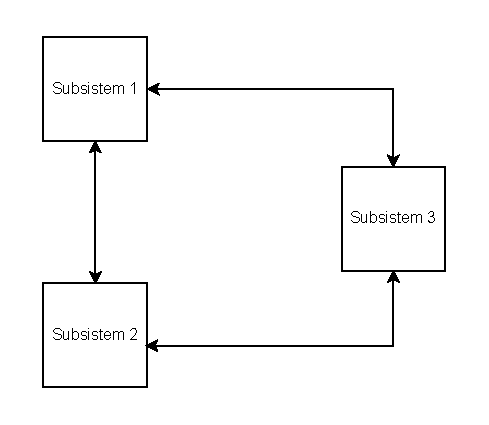
\includegraphics[width=0.8\textwidth]{image//doc/contoh.pdf} % Ganti dengan path diagram Anda
    \caption{Contoh Diagram Arsitektur Sistem Project .}
    \label{fig:elsinta_arch}
\end{figure}

% Ingat untuk menamai gambar Anda dengan format ELx.y yang sudah diatur.

\subsubsection{Contoh: Subsistem Akuisisi Data Sensor (Hardware)}
\textit{Penjelasan: Fokus pada semua komponen fisik yang bertugas mengumpulkan data dari lingkungan. Sebutkan jenis sensor, mikrokontroler, dan modul-modul lain yang terlibat. Jelaskan bagaimana data dikumpulkan dan diproses secara lokal sebelum dikirim. }

Beberapa parameter berikut dapat ditambahkan untuk memperkuat rancangan seperti:

\begin{enumerate}
    \item \textbf{Data Flow Diagram} -- Wajib untuk pembuatan Website.
    \item \textbf{Flowchart/Algoritma} -- Wajib untuk pembuatan program (masing-masing subsistem).
    \item \textbf{Schematic} -- Wajib untuk pembuatan hardware elektronika.
    \item \textbf{PCB Design} -- Wajib.
    \item \textbf{Blok Diagram} -- Wajib untuk arsitektur utama.
    \item \textbf{Desain 3D} -- Wajib untuk menampilkan produk.
    \item \textbf{Skema Web} -- Web yang ditampilkan minimal dalam bentuk skema seperti yang ditunjukkan pada Gambar \ref{fig:web_scheme}.
    \item \textbf{Perhitungan Daya} -- Digunakan untuk memastikan efisiensi dan keamanan sistem tenaga.
    \item \textbf{Persamaan yang Relevan} -- Persamaan matematis yang mendasari sistem yang dibuat, misalnya:
    \begin{equation}
        P = V \times I
    \end{equation}
    \item \textbf{Tabel Pengujian} -- Indikator keberhasilan. Wajib untuk tiap subsistem dan uji gabungan sistem, serta penjelasan mengenai urgensi pengujian tersebut.
    \item \textbf{EL4-Pengujian Sampel Besar} -- Pengujian dalam jumlah sampel yang banyak beserta justifikasinya (waktu dan sumber daya). Data harus disajikan dalam bentuk kurva (tidak hanya tabel) lengkap dengan makna atau analisis dari kurva tersebut.
\end{enumerate}


\begin{figure}
    \centering
    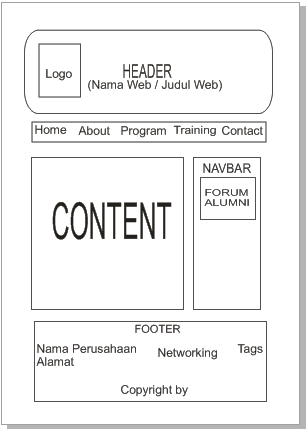
\includegraphics[width=0.5\linewidth]{image/image.png}
    \caption{Contoh skema web}
    \label{fig:web_scheme}
\end{figure}
Subsistem ini bertanggung jawab untuk pengumpulan data kualitas udara dari lingkungan fisik. Komponen utamanya meliputi:
\begin{enumerate}
    \item \textbf{Unit Mikrokontroler:} Menggunakan $\text{ESP32}$ atau $\text{ESP8266}$ (misalnya $\text{NodeMCU}$) sebagai otak utama. Mikrokontroler ini membaca data dari sensor, melakukan pra-pemrosesan (seperti konversi analog ke digital dan kalibrasi awal), dan mengelola komunikasi nirkabel.
    \item \textbf{Modul Sensor Gas:} Terdiri dari berbagai sensor seperti:
    \begin{enumerate}
        \item Sensor $\text{MQ-7}$ untuk Karbon Monoksida ($\text{CO}$).
        \item Sensor $\text{MQ-4}$ atau $\text{MQ-2}$ untuk Metana ($\text{CH}_4$) atau $\text{LPG}$.
        \item Sensor $\text{MH-Z19B}$ atau $\text{SCD30}$ untuk Karbon Dioksida ($\text{CO}_2$).
        \item Sensor $\text{PMS5003}$ atau $\text{SDS011}$ untuk Partikulat Halus ($\text{PM2.5}$).
    \end{enumerate}
    \item \textbf{Modul Sensor Lingkungan Lainnya:} Opsional, dapat mencakup sensor suhu dan kelembaban ($\text{DHT11/DHT22}$) untuk konteks data.
    \item \textbf{Aktuator Lokal:} Terdiri dari kipas $\text{DC}$ atau modul relay untuk ventilasi, serta buzzer atau $\text{LED}$ sebagai indikator peringatan bahaya yang dikontrol langsung oleh mikrokontroler.
\end{enumerate}
Data yang terkumpul dari sensor akan diproses dan difilter di mikrokontroler sebelum dikirim ke subsistem komunikasi.
Contoh  Penulisan Algoritma  di Latex seperti pada Algoritme \autoref{alg:contoh1}:

\begin{algorithm}[H]
\caption{Pembacaan Sensor Suhu dan LED Control}
\label{alg:contoh1}
\begin{algorithmic}[1]
\STATE Inisialisasi pin sensor dan LED
\WHILE{true}
    \STATE Baca nilai suhu dari sensor
    \IF{suhu > 30$^\circ$C}
        \STATE Nyalakan LED
    \ELSE
        \STATE Matikan LED
    \ENDIF
    \STATE Tunggu 1 detik
\ENDWHILE
\end{algorithmic}
\end{algorithm}

Contoh Script di Latex seperti pada \autoref{lst:arduino}: 
\begin{lstlisting}[caption={Contoh Kode Arduino}, label={lst:arduino}]
int led = 13;
int sensor = A0;

void setup() {
  pinMode(led, OUTPUT);
}

void loop() {
  int suhu = analogRead(sensor);
  if (suhu > 600) digitalWrite(led, HIGH);
  else digitalWrite(led, LOW);
  delay(1000);
}

\end{lstlisting}


\subsubsection{Contoh: Subsistem Komunikasi dan Cloud (Software/Network)}
\textit{Penjelasan: Fokus pada bagaimana data dikirim dari perangkat keras ke server/cloud dan bagaimana data tersebut disimpan serta diproses lebih lanjut. Sebutkan protokol komunikasi (\text{MQTT}), platform cloud (\text{AWS IoT, Firebase, Thingspeak}), dan database.}

Subsistem ini bertugas menghubungkan perangkat keras dengan infrastruktur cloud dan mengelola data yang mengalir di dalamnya.
\begin{enumerate}
    \item \textbf{Modul Komunikasi Nirkabel:} Menggunakan modul $\text{WiFi}$ yang terintegrasi pada mikrokontroler ($\text{ESP32/ESP8266}$) untuk konektivitas internet.
    \item \textbf{Protokol Komunikasi \text{IoT}:} Menggunakan \text{MQTT} untuk pengiriman data yang efisien dan ringan dari perangkat ke broker \text{MQTT} di cloud.
    \item \textbf{Platform \text{Cloud} \text{IoT}:} Pilihan platform seperti $\text{Firebase Realtime Database}$, $\text{Thingspeak}$, atau $\text{AWS IoT Core}$ akan digunakan untuk menerima, menyimpan, dan memproses data sensor. Platform ini menyediakan layanan broker \text{MQTT} dan fungsi untuk penyimpanan data.
    \item \textbf{Basis Data (\text{Database}):} Data sensor yang diterima oleh platform cloud akan disimpan dalam basis data (misalnya $\text{Firestore}$ di $\text{Firebase}$ atau $\text{DynamoDB}$ di $\text{AWS}$) untuk data historis dan analisis jangka panjang.
\end{enumerate}
Data di cloud kemudian dapat diakses oleh subsistem visualisasi dan kontrol dari mana saja.

\subsubsection{Contoh: Subsistem Visualisasi dan Kontrol Pengguna (Software/Aplikasi) (Optional / Jika ada}
\textit{Penjelasan: Fokus pada bagian yang berinteraksi langsung dengan pengguna. Jelaskan antarmuka pengguna (\emph{dashboard} web/mobile), fungsinya (menampilkan data, mengatur threshold, melihat histori), dan bagaimana pengguna dapat memberikan perintah balik ke sistem (jika ada).}

Subsistem ini menyediakan antarmuka bagi pengguna untuk memantau kualitas udara, menganalisis data, dan mengonfigurasi sistem.
\begin{enumerate}
    \item \textbf{\emph{Dashboard} Berbasis Web/Mobile:} Aplikasi web (misalnya dengan $\text{React}$ atau $\text{Vue.js}$) atau aplikasi mobile (misalnya dengan $\text{Flutter}$ atau $\text{React Native}$) yang berfungsi sebagai antarmuka pengguna utama.
    \item \textbf{Visualisasi Data Real-time:} Menampilkan grafik dan nilai numerik dari semua parameter sensor secara real-time yang diunduh dari cloud.
    \item \textbf{Analisis Data Historis:} Menyediakan fitur untuk melihat data sensor historis dalam periode waktu tertentu, membantu identifikasi tren dan pola.
    \item \textbf{Konfigurasi Sistem:} Memungkinkan pengguna untuk mengatur ambang batas (threshold) konsentrasi gas untuk aktivasi aktuator dan alarm, serta pengaturan parameter sistem lainnya.
    \item \textbf{Sistem Notifikasi:} Menampilkan peringatan visual di dashboard dan mengirimkan notifikasi (email/pesan) saat ambang batas bahaya terlampaui.
    \item \textbf{Kontrol Aktuator Jarak Jauh (Opsional):} Memungkinkan pengguna untuk secara manual mengaktifkan/menonaktifkan aktuator (misalnya kipas) dari dashboard, memberikan fleksibilitas tambahan dalam pengendalian.
\end{enumerate}
Subsistem ini menjadi jembatan antara data teknis dari perangkat keras dan kebutuhan informasi serta kontrol dari pengguna akhir.

\textbf{Project ELSINTA} adalah sebuah sistem terintegrasi untuk pemantauan dan pengendalian kualitas udara dalam ruangan secara otomatis dan real-time. Sistem ini dirancang untuk mendeteksi berbagai jenis gas berbahaya dan partikulat, serta secara proaktif merespons kondisi udara yang memburuk melalui aktivasi aktuator. \textbf{Project ELSINTA} terdiri dari unit perangkat keras yang dilengkapi multi-sensor dan mikrokontroler, platform komunikasi nirkabel ($\text{WiFi}$), serta dashboard berbasis web/mobile untuk visualisasi data dan konfigurasi sistem. Tujuan utamanya adalah menciptakan lingkungan dalam ruangan yang lebih aman dan sehat dengan biaya yang efektif.

\subsection{\MainFeaturesTitle}
\textit{Penjelasan: Daftarkan fitur-fitur utama yang akan disediakan oleh Project anda. Gunakan poin-poin yang jelas dan spesifik. Fokus pada apa yang dapat dilakukan oleh sistem yang tim buat.}

\textbf{Contoh:} Berikut adalah fitur-fitur kunci yang akan diimplementasikan dalam \textbf{Project ELSINTA}:
\begin{enumerate}
    \item \textbf{Pemantauan Multi-Sensor Gas dan Partikulat:} Integrasi sensor untuk mendeteksi Karbon Monoksida ($\text{CO}$), Metana/LPG ($\text{CH}_4$), Karbon Dioksida ($\text{CO}_2$), dan Partikulat Halus ($\text{PM2.5}$).
    \item \textbf{Kontrol Aktif Otomatis:} Sistem akan secara otomatis mengendalikan aktuator seperti kipas/ventilasi dan alarm suara/visual (misalnya lampu indikator $\text{LED}$) berdasarkan ambang batas konsentrasi gas yang terdeteksi.
    \item \textbf{Komunikasi Nirkabel (\text{IoT}) dan Akses Real-time:} Penggunaan modul $\text{WiFi}$ untuk mengirimkan data sensor ke cloud, memungkinkan pemantauan kualitas udara secara real-time dari mana saja melalui internet.
    \item \textbf{Platform Visualisasi Data (Dashboard Web/Mobile):} Menyediakan antarmuka grafis yang intuitif (dashboard) untuk menampilkan data sensor secara real-time, data historis, serta status aktuator.
    \item \textbf{Notifikasi dan Peringatan Dini:} Mengirimkan notifikasi (misalnya, melalui email atau pesan aplikasi) kepada pengguna ketika ambang batas gas berbahaya terlampaui atau ada anomali.
    \item \textbf{Konfigurasi Ambang Batas Adaptif:} Pengguna dapat mengatur atau menyesuaikan ambang batas (threshold) konsentrasi gas untuk aktivasi alarm dan aktuator melalui dashboard.
    \item \textbf{Penyimpanan Data Historis:} Data sensor akan disimpan di cloud untuk analisis tren jangka panjang dan pelaporan.
\end{enumerate}

\subsection{\AdvantagesTitle}
\textit{Penjelasan: Di bagian ini, bandingkan Project anda dengan solusi eksisting yang Anda bahas di \textbf{State of the Art} dan \textbf{Gap Analysis}. Tekankan mengapa proyek Anda lebih baik, lebih inovatif, atau lebih relevan, dengan merujuk kembali ke "celah" yang berhasil Anda isi. Fokus pada nilai tambah yang ditawarkan.}

\textbf{Contoh: } Project ELSINTA menawarkan beberapa keunggulan signifikan dibandingkan solusi pemantauan dan pengendalian kualitas udara yang sudah ada di pasaran atau prototipe penelitian terdahulu:
\begin{enumerate}
    \item \textbf{Solusi Holistik dan Terintegrasi dengan Biaya Efektif:} Berbeda dengan produk komersial mahal yang fokus pada beberapa parameter, Project ELSINTA mengintegrasikan pemantauan multi-gas berbahaya dan partikulat dengan sistem kontrol aktif dan fitur \text{IoT} yang komprehensif, namun dengan biaya implementasi yang jauh lebih terjangkau.
    \item \textbf{Kontrol Aktif Adaptif Multi-Aktuator:} Banyak solusi hanya memberikan peringatan atau kontrol terbatas. Project ELSINTA dirancang dengan algoritma kontrol cerdas yang dapat mengaktifkan berbagai aktuator (kipas, alarm) secara dinamis berdasarkan jenis dan tingkat ancaman gas, memberikan respons yang lebih efektif dan otomatis.
    \item \textbf{Fokus pada Akurasi dan Keandalan Data:} Melalui implementasi metode kalibrasi awal dan koreksi data, Project ELSINTA berupaya mengatasi masalah akurasi sensor \text{MQ}-series yang sering menjadi kelemahan prototipe low-cost, sehingga menghasilkan data yang lebih andal untuk pengambilan keputusan.
    \item \textbf{Kustomisasi dan Skalabilitas Lingkungan:} Sistem ini dirancang untuk mudah dikonfigurasi dan diadaptasi sesuai kebutuhan spesifik lingkungan ruangan, mulai dari ambang batas alarm hingga jenis aktuator. Ini memberikan fleksibilitas yang lebih besar dibandingkan produk "kotak hitam" yang kaku.
    \item \textbf{Analisis Data Jangka Panjang yang Didukung IoT:} Dengan penyimpanan data historis di cloud dan dashboard interaktif, Project ELSINTA tidak hanya memantau secara real-time, tetapi juga memungkinkan pengguna untuk menganalisis tren, mengidentifikasi pola, dan mengoptimalkan strategi manajemen kualitas udara dari waktu ke waktu.
\end{enumerate}

\subsection{\AlternativeDesignTitle}

\subsection{\JustificationTitle}
\textit{Bagian ini bertujuan untuk menjustifikasi pemilihan komponen arsitektur utama Project dengan menganalisis solusi-solusi atau komponen alternatif yang sempat dipertimbangkan. Untuk setiap alternatif, jelaskan kelemahan spesifiknya yang menyebabkan penolakan, sehingga memperkuat argumen bahwa solusi yang dipilih adalah yang paling optimal berdasarkan kriteria biaya, kinerja, dan kompleksitas.}

\textbf{Contoh}: Selama tahap desain, beberapa solusi alternatif telah dipertimbangkan sebelum memutuskan untuk mengembangkan arsitektur \text{IoT} berbasis $\text{ESP32}$ dan $\text{MQTT}$. Alternatif-alternatif tersebut antara lain:

\subsubsection*{Alternatif 1: Sistem Pemantauan Berbasis Jaringan Kabel (\text{RS485})}
\begin{enumerate}
    \item \textbf{Deskripsi:} Alih-alih menggunakan $\text{WiFi}$, data sensor akan dikirim menggunakan koneksi kabel $\text{RS485}$ ke unit pusat (Gateway) yang kemudian mengirimkan data ke cloud.
    \item \textbf{Alasan Penolakan:} Meskipun $\text{RS485}$ menawarkan keandalan tinggi dan kekebalan kebisingan yang baik (teknis), ini memerlukan instalasi kabel yang kompleks, mahal, dan tidak fleksibel, sehingga bertentangan dengan tujuan proyek untuk menciptakan solusi yang mudah dipasang (\textit{plug-and-play}) dan efektif biaya.
\end{enumerate}

\subsubsection*{Alternatif 2: Sistem Pemantauan Lokal Tanpa \text{Cloud}}
\begin{enumerate}
    \item \textbf{Deskripsi:} Sistem hanya akan menggunakan mikrokontroler dan layar $\text{LCD}$ lokal untuk menampilkan data dan mengaktifkan alarm/kipas. Tidak ada koneksi internet, dashboard, atau penyimpanan data historis.
    \item \textbf{Alasan Penolakan:} Solusi ini tidak memenuhi kebutuhan kunci pasar akan akses data real-time dan analisis historis. Meskipun biayanya sangat rendah, kelemahan ini secara signifikan mengurangi dampak dan nilai tambah (\textit{value proposition}) proyek, terutama dalam konteks pelaporan dan manajemen risiko.
\end{enumerate}

\subsubsection*{Alternatif 3: Penggunaan Mikrokontroler Raspberry Pi atau Single-Board Computer}
\begin{enumerate}
    \item \textbf{Deskripsi:} Menggunakan $\text{Raspberry Pi}$ untuk memproses data sensor dan menjalankan web server lokal.
    \item \textbf{Alasan Penolakan:} $\text{Raspberry Pi}$ menawarkan kemampuan komputasi berlebihan (overkill) untuk tugas pembacaan sensor sederhana dan meningkatkan konsumsi daya secara drastis. Selain itu, biaya komponen menjadi lebih mahal dan tidak sejalan dengan tujuan utama proyek untuk menyediakan solusi yang efektif biaya. Pilihan $\text{ESP32}$ dianggap sudah memadai untuk kapabilitas \text{IoT} dan kontrol.
\end{enumerate}


\section{\ImplementationPlanTitle}

Bagian ini menguraikan rencana strategis dan operasional untuk pengembangan project tim,  yang mencakup pembagian pekerjaan, jadwal implementasi, dan alokasi tanggung jawab tim untuk memastikan proyek berjalan sesuai tujuan dan diselesaikan secara efisien.

\subsection{\WBSTitle}
\textit{Penjelasan: \text{WBS} adalah dekomposisi hierarkis dari keseluruhan pekerjaan proyek menjadi komponen-komponen yang lebih kecil dan mudah dikelola. Mulailah dari fase utama (misalnya, Perencanaan, Desain, Implementasi, Pengujian, Dokumentasi) kemudian pecah lagi menjadi tugas-tugas yang lebih spesifik. Setiap tugas harus memiliki deliverable yang jelas.}

 Work Breakdown Structure (WBS) Project  membagi pekerjaan menjadi fase-fase dan tugas-tugas yang terdefinisi dengan baik untuk memudahkan perencanaan, pelacakan, dan pengelolaan proyek.

\subsubsection*{Contoh Struktur \text{WBS}:}
\begin{enumerate}
    \item \textbf{Fase 1: Perencanaan dan Analisis (Minggu 1-2)}
    \begin{enumerate}
        \item \text{WBS 1.1}: Analisis Kebutuhan Sistem
        \item \text{WBS 1.2}: Studi Literatur dan Kompetitor
        \item \text{WBS 1.3}: Perancangan Arsitektur Sistem Global
    \end{enumerate}
    \item \textbf{Fase 2: Desain Sistem (Minggu 3-5)}
    \begin{enumerate}
        \item \text{WBS 2.1}: Desain Skematik Hardware (Sensor, Mikrokontroler, Aktuator)
        \item \text{WBS 2.2}: Desain PCB (Opsional, jika membuat PCB kustom)
        \item \text{WBS 2.3}: Desain Database dan API \text{Cloud}
        \item \text{WBS 2.4}: Desain Antarmuka Pengguna (Dashboard Web/Mobile)
        \item \text{WBS 2.5}: Desain Algoritma Kontrol dan Kalibrasi
    \end{enumerate}
    \item \textbf{Fase 3: Implementasi (Minggu 6-10)}
    \begin{enumerate}
        \item \text{WBS 3.1}: Perakitan Hardware dan Wiring
        \item \text{WBS 3.2}: Pengembangan Firmware Mikrokontroler (Pembacaan sensor, Kontrol Aktuator)
        \item \text{WBS 3.3}: Integrasi Komunikasi \text{IoT} (\text{MQTT}, Koneksi \text{Cloud})
        \item \text{WBS 3.4}: Pengembangan Backend Aplikasi (\text{API}, Logika Bisnis)
        \item \text{WBS 3.5}: Pengembangan Frontend Aplikasi (Dashboard Web/Mobile)
    \end{enumerate}
    \item \textbf{Fase 4: Pengujian dan Kalibrasi (Minggu 11-13)}
    \begin{enumerate}
        \item \text{WBS 4.1}: Pengujian Fungsionalitas Hardware
        \item \text{WBS 4.2}: Kalibrasi Sensor dan Validasi Akurasi
        \item \text{WBS 4.3}: Pengujian Integrasi Sistem End-to-End
        \item \text{WBS 4.4}: Pengujian Performa dan Stabilitas Sistem
        \item \text{WBS 4.5}: Pengujian Antarmuka Pengguna (\text{UAT})
    \end{enumerate}
    \item \textbf{Fase 5: Dokumentasi dan Pelaporan (Minggu 14-16)}
    \begin{enumerate}
        \item \text{WBS 5.1}: Penulisan Laporan Akhir
        \item \text{WBS 5.2}: Pembuatan Buku Panduan Pengguna
        \item \text{WBS 5.3}: Persiapan Presentasi dan Poster
    \end{enumerate}
\end{enumerate}

\subsection{\TimelineTitle}
\textit{Penjelasan: Bagian ini harus menampilkan jadwal proyek dalam bentuk Gantt Chart. Gantt Chart memvisualisasikan durasi setiap tugas dari \text{WBS} dan ketergantungan antar tugas. Karena Anda membuat buku panduan, Anda bisa menyertakan contoh Gantt Chart atau menjelaskan struktur data yang akan digunakan untuk membuat Gantt Chart.}



\subsubsection*{Struktur Umum Timeline:}
Setiap fase dan tugas yang dijelaskan dalam \text{WBS} akan dialokasikan pada linimasa proyek. Umumnya, proyek Capstone Design/Tugas Akhir memakan waktu 4-6 bulan (16-24 minggu).
\begin{enumerate}
    \item \textbf{Minggu 1-2:} Perencanaan dan Analisis
    \item \textbf{Minggu 3-5:} Desain Sistem
    \item \textbf{Minggu 6-10:} Implementasi
    \item \textbf{Minggu 11-13:} Pengujian dan Kalibrasi
    \item \textbf{Minggu 14-16:} Dokumentasi dan Pelaporan
\end{enumerate}
\textit{Catatan: Gantt Chart harus mencakup nama tugas, durasi, tanggal mulai/akhir, dan ketergantungan antar tugas. Warna atau simbol dapat digunakan untuk menunjukkan status tugas.}

\subsection{\TeamDivisionTitle}
\textit{Penjelasan: Jelaskan alokasi tanggung jawab masing-masing anggota tim untuk setiap tugas atau subsistem utama. Ini menunjukkan bagaimana beban kerja didistribusikan dan siapa yang bertanggung jawab atas bagian tertentu dari proyek.}

Pembagian tugas tim sangat krusial untuk efisiensi dan akuntabilitas. Setiap anggota tim akan memiliki peran dan tanggung jawab yang jelas sesuai dengan keahliannya.

\subsubsection*{Contoh Pembagian Tugas (untuk Tim 2-3 Orang):}
\begin{enumerate}
    \item \textbf{Ketua Tim (Mahasiswa A):}
    \begin{enumerate}
        \item Koordinator Proyek dan Komunikasi.
        \item Perancangan Arsitektur Sistem Global dan Manajemen Proyek.
        \item Pengembangan Backend Aplikasi dan Database \text{Cloud}.
        \item Pengujian Integrasi Sistem.
    \end{enumerate}
    \item \textbf{Anggota Tim 1 (Mahasiswa B):}
    \begin{enumerate}
        \item Perancangan dan Implementasi Hardware (Sensor, Mikrokontroler, Aktuator).
        \item Pengembangan Firmware Mikrokontroler dan Algoritma Kontrol.
        \item Kalibrasi Sensor dan Pengujian Hardware.
    \end{enumerate}
    \item \textbf{Anggota Tim 2 (Mahasiswa C - Opsional):}
    \begin{enumerate}
        \item Pengembangan Frontend Aplikasi (\emph{Dashboard} Web/Mobile) dan \emph{User Experience}.
        \item Perancangan dan Implementasi Sistem Notifikasi.
        \item Dokumentasi Teknis dan Panduan Pengguna.
    \end{enumerate}
\end{enumerate}
\textit{Catatan: Pembagian tugas harus spesifik untuk proyek Anda dan disetujui oleh Dosen Pembimbing.}


\subsection{\SystemTestingTitle}


Sub-bab \textbf{Pengujian Sistem} mendokumentasikan proses sistematis yang dilakukan untuk memverifikasi bahwa implementasi solusi teknis telah selesai dengan benar dan memvalidasi bahwa sistem tersebut memenuhi kebutuhan fungsional dan non-fungsional yang ditetapkan.

Fokus utama bagian ini adalah menjawab pertanyaan: Apakah sistem berjalan sebagaimana mestinya dan apakah sistem melakukan apa yang seharusnya dilakukan?
Jelaskan juga mengapa pengujian ini perlu dilakukan dan  parameter apa yang digunakan dalam pengujian, termasuk jenis-jenis pengujian yang dilakukan. Kriteria keberhasilan yang ditetapkan diilustrasikan dalam Tabel~\ref{tab:kriteria_pengujian}.

\begin{longtable}{|c|p{5cm}|p{8cm}|}
    \caption{Contoh Kriteria Keberhasilan Pengujian Sistem Elektronika}
    \label{tab:kriteria_pengujian_elektro}
    \\ % Baris kosong untuk memisahkan caption dari header

    \hline
    \textbf{No.} & \textbf{Parameter Pengujian} & \textbf{Kriteria Keberhasilan} \\
    \hline
    \endhead % Header akan diulang di setiap halaman

    \hline
    1 & Pengujian Keluaran Tegangan (Output Voltage) & Tegangan keluaran harus berada dalam rentang $4.8 \text{V} \leq V_{out} \leq 5.2 \text{V}$ \\
    \hline
    2 & Pengujian Akurasi Sensor Suhu ($\text{LM35}$) & Penyimpangan hasil pengukuran $\leq 0.5^\circ \text{C}$ dari referensi standar \\
    \hline
    3 & Konsumsi Arus (\textit{Idle State}) & Konsumsi arus pada kondisi diam $\leq 50 \text{mA}$ \\
    \hline
    4 & Waktu Respons Aktor (\textit{Relay}) & Waktu tunda antara sinyal input dan aktivasi aktor $\leq 100$ milidetik \\
    \hline
    5 & Keandalan Koneksi Nirkabel ($\text{Wi-Fi}$) & Tingkat keberhasilan transmisi data ke server $\geq 98\%$ \\
    \hline
    6 & Daya Tahan Baterai (\textit{Low-Power Mode}) & Sistem harus mampu beroperasi selama $\geq 24$ jam tanpa pengisian ulang \\
    \hline
\end{longtable}


 tambahkan tabel pengujian integrasi sistem
 
\section{\RiskAssessmentTitle}

Bagian ini mengidentifikasi potensi risiko yang dapat memengaruhi keberhasilan project anda, mengevaluasi dampaknya, dan merumuskan strategi mitigasi untuk mengurangi kemungkinan dan/atau konsekuensi dari risiko tersebut.

\subsection{\TechFinancialRiskTitle}
\textit{Penjelasan: Klasifikasikan risiko ke dalam kategori yang berbeda. Identifikasi risiko spesifik yang mungkin terjadi dalam pengembangan Project anda. Untuk setiap risiko, jelaskan sifatnya dan potensi dampaknya pada proyek.}

\subsubsection*{Technical Risk}
Risiko yang terkait dengan aspek teknologi, implementasi, dan fungsionalitas sistem.
\begin{enumerate}
    \item \textbf{Akurasi dan Stabilitas Sensor Rendah:} Sensor low-cost ($\text{MQ}$-series) mungkin tidak memberikan data yang cukup akurat atau stabil dalam jangka panjang atau pada kondisi lingkungan yang dinamis, memengaruhi keandalan sistem.
    \item \textbf{Kompatibilitas Hardware/Software:} Kesulitan dalam integrasi berbagai modul sensor, mikrokontroler, atau library perangkat lunak, menyebabkan keterlambatan pengembangan.
    \item \textbf{Konektivitas \text{IoT} Tidak Stabil:} Gangguan pada koneksi \text{WiFi} atau masalah dengan layanan cloud dapat menyebabkan hilangnya data atau keterlambatan notifikasi.
    \item \textbf{Kesulitan Kalibrasi:} Proses kalibrasi multi-sensor yang kompleks dan memakan waktu, terutama tanpa peralatan kalibrasi standar.
\end{enumerate}

\subsubsection*{Financial Risk}
Risiko yang berkaitan dengan anggaran dan sumber daya keuangan proyek.
\begin{enumerate}
    \item \textbf{Pembengkakan Biaya Komponen:} Harga komponen elektronik yang berfluktuasi atau kebutuhan akan komponen yang lebih mahal dari estimasi awal.
    \item \textbf{Biaya Layanan \text{Cloud} Tak Terduga:} Jika menggunakan layanan cloud berbayar, biaya dapat melebihi anggaran jika penggunaan data atau fitur melebihi ekspektasi.
\end{enumerate}

\subsubsection*{User Acceptance Risk}
Risiko yang berkaitan dengan persepsi, kepuasan, dan adopsi sistem oleh pengguna akhir.
\begin{enumerate}
    \item \textbf{Antarmuka Pengguna Kurang Intuitif:} Dashboard yang rumit atau tidak mudah digunakan dapat mengurangi minat pengguna untuk memantau data secara rutin.
    \item \textbf{Notifikasi Berlebihan/Tidak Akurat:} Sistem yang sering memberikan peringatan palsu (\emph{false alarms}) atau notifikasi yang tidak relevan dapat menyebabkan kelelahan peringatan (\emph{alarm fatigue}) dan mengurangi kepercayaan pengguna.
    \item \textbf{Kurangnya Edukasi Pengguna:} Pengguna tidak memahami cara kerja sistem atau pentingnya pemantauan kualitas udara, sehingga adopsi rendah.
\end{enumerate}

\subsection{\RiskMitigationTitle}
\textit{Penjelasan: Untuk setiap risiko yang teridentifikasi, jelaskan tindakan spesifik yang akan diambil untuk mengurangi kemungkinan terjadinya risiko atau meminimalkan dampaknya jika risiko tersebut terjadi.}

\subsubsection*{Strategi Mitigasi Risiko:}
\begin{enumerate}
    \item \textbf{Mitigasi Risiko Teknis:}
    \begin{enumerate}
        \item \textbf{Akurasi Sensor:} Melakukan pengujian ekstensif pada berbagai kondisi, mengimplementasikan algoritma filter data dan kalibrasi perangkat lunak. Lakukan kalibrasi dengan teknik linear atau nonlinear ketika akurasi tidak sesuai.
        \item \textbf{Kompatibilitas Hardware/Software:} Melakukan prototyping cepat untuk mengidentifikasi dan menyelesaikan masalah kompatibilitas sejak awal. Menggunakan library dan framework yang terbukti stabil.
        \item \textbf{Konektivitas \text{IoT} Stabil:} Mengimplementasikan mekanisme reconnection otomatis dan buffering data lokal pada mikrokontroler. Memilih platform cloud dengan reputasi stabilitas tinggi.
        \item \textbf{Kesulitan Kalibrasi:} Mengembangkan prosedur kalibrasi sederhana yang dapat dilakukan on-site dengan panduan jelas, atau menggunakan metode kalibrasi adaptif berbasis data.
    \end{enumerate}
    \item \textbf{Mitigasi Risiko Finansial:}
    \begin{enumerate}
        \item \textbf{Biaya Komponen:} Melakukan riset pasar menyeluruh untuk mendapatkan harga komponen terbaik. Menyediakan buffer anggaran sebesar 10-15\% untuk biaya tak terduga.
        \item \textbf{Biaya Layanan \text{Cloud}:} Memilih platform cloud dengan paket gratis atau biaya rendah yang sesuai dengan estimasi penggunaan awal. Memonitor penggunaan sumber daya cloud secara berkala.
    \end{enumerate}
    \item \textbf{Mitigasi Risiko Penerimaan Pengguna:}
    \begin{enumerate}
        \item \textbf{Antarmuka Pengguna:} Melibatkan calon pengguna dalam fase desain \emph{dashboard} (\text{User-Centered Design}). Melakukan \text{UAT} dan mengumpulkan feedback untuk iterasi desain.
        \item \textbf{Notifikasi Akurat:} Mengimplementasikan algoritma filter kebisingan pada data sensor untuk mengurangi false alarms. Menyediakan opsi konfigurasi sensitivitas notifikasi bagi pengguna.
        \item \textbf{Edukasi Pengguna:} Menyediakan buku panduan pengguna yang komprehensif, video tutorial, dan sesi pelatihan singkat jika diperlukan.
    \end{enumerate}
\end{enumerate}

---

\section{\FinancialAnalysisTitle}

Bagian ini menyajikan estimasi biaya yang terkait dengan pengembangan dan implementasi \textbf{Project }, serta analisis manfaat-biaya. Analisis finansial ini membantu dalam menilai kelayakan ekonomi proyek.

\subsection{\CostEstimationTitle}
\textit{Penjelasan: Rincikan komponen biaya utama yang akan dikeluarkan selama pengembangan Project. Kategorikan biaya-biaya ini untuk memberikan gambaran yang jelas. Fokus pada biaya hardware dan software.}

Estimasi biaya ini mencakup pengeluaran utama yang diperlukan untuk mengembangkan prototipe Project.

\subsubsection*{Contoh Estimasi Biaya:}
\begin{enumerate}
    \item \textbf{Biaya Hardware (\text{Unit Prototipe}):}
    \begin{enumerate}
        \item Mikrokontroler ($\text{ESP32/ESP8266}$): 2 unit @ \text{Rp 50.000} = \text{Rp 100.000}
        \item Sensor Gas ($\text{MQ-7, MQ-4, MH-Z19B, PMS5003}$): Total 4 sensor @ rata-rata \text{Rp 150.000} = \text{Rp 600.000}
        \item Aktuator (Kipas $\text{DC}$, Relay, Buzzer, $\text{LED}$): Total \text{Rp 100.000}
        \item Power Supply, Kabel, PCB, Casing Prototipe: Total \text{Rp 200.000}
        \item \textbf{Subtotal Hardware:} \text{Rp 1.000.000}
    \end{enumerate}
    \item \textbf{Biaya Software/Layanan (\text{Jika Berlangganan/Premium}):}
    \begin{enumerate}
        \item Layanan \text{Cloud IoT} (misalnya paket premium $\text{Thingspeak}$ atau \text{AWS IoT}): Estimasi \text{Rp 0 - Rp 100.000/bulan} (untuk skala prototipe seringkali gratis).
        \item Domain/Hosting Web (jika dashboard self-hosted): Estimasi \text{Rp 0 - Rp 50.000/bulan}.
        \item \textbf{Subtotal Software/Layanan:} \text{Rp 0 - Rp 300.000} (untuk 3 bulan pengembangan).
    \end{enumerate}
    \item \textbf{Biaya Lain-lain (Penelitian, Transportasi, Dokumentasi):}
    \begin{enumerate}
        \item Biaya Referensi/Jurnal, Fotokopi, Print: \text{Rp 150.000}
        \item Transportasi (jika ada kunjungan): \text{Rp 100.000}
        \item \textbf{Subtotal Lain-lain:} \text{Rp 250.000}
    \end{enumerate}
    \item \textbf{Total Estimasi Biaya Proyek:} \text{Rp 1.000.000} + \text{Rp 300.000} + \text{Rp 250.000} = \textbf{Rp 1.550.000}
\end{enumerate}
\textit{Catatan: Estimasi ini adalah contoh. Biaya sebenarnya harus disesuaikan dengan harga pasar saat ini dan kebutuhan spesifik proyek Anda.}

\subsection{\CostBenefitTitle}
\textit{Penjelasan: Bandingkan total estimasi biaya dengan manfaat ekonomi dan non-ekonomi yang diharapkan dari Projec. Jelaskan mengapa manfaat (misalnya, peningkatan keselamatan, efisiensi operasional, potensi komersial) jauh melampaui biaya investasi, terutama dalam jangka panjang.}

Analisis manfaat-biaya mengevaluasi apakah manfaat yang diperoleh dari Project ELSINTA sepadan dengan biaya yang dikeluarkan.

\subsubsection*{Manfaat Finansial dan Non-Finansial:}
\begin{enumerate}
    \item \textbf{Manfaat Utama (\emph{Non-Finansial, tapi Bernilai Tinggi}):} Peningkatan keselamatan jiwa dan aset, peningkatan kesehatan dan produktivitas lingkungan kerja/belajar. Pencegahan insiden gas berbahaya dapat menghindari kerugian finansial yang jauh lebih besar (misalnya, biaya pengobatan, denda regulasi, kerusakan reputasi).
    \item \textbf{Manfaat Finansial Langsung:} Penghematan dari penggunaan solusi low-cost dibandingkan produk komersial ($\text{Rp 1.550.000}$ vs. \text{Rp 5.000.000 - Rp 20.000.000}). Potensi penghematan biaya energi melalui kontrol ventilasi yang efisien (jangka panjang).
    \item \textbf{Manfaat Potensial (Jangka Panjang):} Potensi komersialisasi produk yang dapat menciptakan nilai ekonomi. Proyek ini juga memberikan nilai edukasi dan penelitian yang tak ternilai bagi institusi.
\end{enumerate}

\subsubsection*{Kesimpulan Analisis Manfaat-Biaya:}
Meskipun Project ini memerlukan investasi awal, manfaat yang ditawarkan, terutama dalam aspek keselamatan, kesehatan, dan potensi efisiensi operasional, jauh melampaui biaya yang dikeluarkan. Pencegahan satu insiden kebocoran gas dapat menghemat kerugian finansial yang signifikan, menjadikan investasi ini sangat berharga. Selain itu, nilai akademik dan potensi pengembangan lanjutan memberikan justifikasi yang kuat untuk implementasi proyek ini.

\section{\ReferencesTitle}
Daftar pustaka ditulis sesuai standar IEEE, sebaiknya gunakan Citation tools seperti Mendeley, Zotero dll. Semuanya dimasukkan atau replace file pustaka.bib.

Contoh format IEEE:  
\renewcommand{\refname}{}      % Hapus judul default "Pustaka"
\bibliographystyle{IEEEtran} % Menggunakan style sitasi IEEE
\bibliography{pustaka}    % Memanggil file pustaka.bib




\section{\AbbrevTitle}

% longtable tidak menggunakan lingkungan table[] di sekitarnya.
% Perintah \begin{longtable} langsung menggantikan \begin{table}\begin{tabular}
\begin{longtable}{|p{4cm}|p{11cm}|} % Lebar kolom ditetapkan agar teks wrap
    \caption{Daftar Singkatan (Abbreviations)} \label{tab:abbreviations3} \\
    \hline
    \textbf{Abbreviation} & \textbf{Definition} \\
    \hline
    \endhead % Mengakhiri baris header yang akan diulang di setiap halaman
    
    \hline 
    \multicolumn{2}{|r|}{Lanjutan di halaman berikutnya...} \\ 
    \endfoot % Footer untuk semua halaman kecuali yang terakhir
    
    \hline
    \endlastfoot % Footer untuk halaman terakhir (kosong)

    % --- Isi Tabel ---
    IoT & Internet of Things \\
    \hline
    KPI & Key Performance Indicator \\
    \hline
    ROI & Return on Investment \\
    \hline
    WBS & Work Breakdown Structure \\
    \hline
    SWOT & Strengths, Weaknesses, Opportunities, Threats \\
    \hline
    BMC & Business Model Canvas \\
    \hline
    IEEE & Institute of Electrical and Electronics Engineers \\
    \hline
    ISO & International Organization for Standardization \\
    \hline
    G-MoCo & Gas Quality Monitoring and Controlling (Nama Proyek Anda) \\
    \hline
    CO & Carbon Monoxide \\
    \hline
    CH$_4$ & Methane (atau LPG) \\
    \hline
    PM2.5 & Particulate Matter 2.5 \\
    \hline
    
    % Tambahkan lebih banyak baris di sini untuk memicu pemisahan halaman
    % ... (Tambahkan entri lain jika tabel perlu memanjang)

\end{longtable}


\end{document}